%%%%%%%%%%%%%%%%%%%%%% Generalities %%%%%%%%%%%%%%%%%%5
\documentclass[11pt,fleqn]{article}
\usepackage[paper=a4paper]
  {geometry}

\pagestyle{plain}
\pagenumbering{arabic}
%%%%%%%%%%%%%%%%%%%%%%%%%%%%%%%%
% esto tiene que estar, en este orden...
\usepackage[small]{titlesec}
\usepackage{paragraphs}
\usepackage{hyperref}
\usepackage{amsthm,thmtools}

%\linespread{1.2}
\setlength{\parskip}{1.2ex}

\usepackage[latin1,utf8]{inputenc}
\usepackage[spanish,english]{babel}
\usepackage{enumerate}
\usepackage{mathpazo}
\usepackage{euler}
\usepackage[alphabetic,initials]{amsrefs}
\usepackage{amsfonts,amssymb,amsmath}
\usepackage{dsfont}
\usepackage{mathtools}
\usepackage{graphicx}
\usepackage[poly,arrow,curve,matrix]{xy}
\usepackage{wrapfig}
%\swapnumbers

% numbered versions
\declaretheoremstyle[headformat=swapnumber, spaceabove=\paraskip,
bodyfont=\itshape]{mystyle}
\declaretheorem[name=Lemma, sibling=para, style=mystyle]{Lemma}
\declaretheorem[name=Proposici\'on, sibling=para, style=mystyle]{Proposition}
\declaretheorem[name=Theorem, sibling=para, style=mystyle]{Theorem}
\declaretheorem[name=Corolllary, sibling=para, style=mystyle]{Corollary}
\declaretheorem[name=Definition, sibling=para, style=mystyle]{Definition}

% unnumbered versions
\declaretheoremstyle[numbered=no, spaceabove=\paraskip,
bodyfont=\itshape]{mystyle-empty}
\declaretheorem[name=Lemma, style=mystyle-empty]{Lemma*}
\declaretheorem[name=Proposici\'on, style=mystyle-empty]{Proposition*}
\declaretheorem[name=Theorem, style=mystyle-empty]{Theorem*}
\declaretheorem[name=Corollary, style=mystyle-empty]{Corollary*}
\declaretheorem[name=Definition, style=mystyle-empty]{Definition*}

% plain style
\declaretheoremstyle[
        headformat={{\bfseries\NUMBER.}{\itshape\NAME}\NOTE\ignorespaces},
        spaceabove=\paraskip, 
        headpunct={.},
        headfont=\itshape,
        bodyfont=\normalfont
        ]{mystyle-plain}
\declaretheorem[sibling=para, style=mystyle-plain]{Example}
\declaretheorem[sibling=para, style=mystyle-plain]{Remark}

% proofs, just as in amsthm but with adapted spacing
\makeatletter
\renewenvironment{proof}[1][Demostraci\'on]{\par
  \pushQED{\qed}%
  \normalfont \topsep.75\paraskip\relax
  \trivlist
  \item[\hskip\labelsep
        \itshape
    #1\@addpunct{.}]\ignorespaces
}{%
  \popQED\endtrivlist\@endpefalse
}
\makeatother

%%%%%%%%%%%%%%%%%%%%%%%%%%% The usual stuff%%%%%%%%%%%%%%%%%%%%%%%%%
\newcommand\NN{\mathbb N}
\newcommand\CC{\mathbb C}
\newcommand\QQ{\mathbb Q}
\newcommand\RR{\mathbb R}
\newcommand\ZZ{\mathbb Z}
\newcommand\FF{\mathbb F}

\newcommand\maps{\longmapsto}
\newcommand\ot{\otimes}
\renewcommand\to{\longrightarrow}
\renewcommand\phi{\varphi}
\newcommand\stack[2]{\genfrac{}{}{0pt}{2}{#1}{#2}}
\newcommand\uu[1]{\underline{#1}}

%%%%%%%%%%%%%%%%%%%%%%%%% Specific notation %%%%%%%%%%%%%%%%%%%%%%%%%

\newcommand\A{\mathcal A}
\newcommand\B{\mathcal B}
\renewcommand\L{\mathcal L}
\newcommand\R{\mathcal R}
\newcommand\F{\mathcal F}
\renewcommand\O{\mathcal O}
\newcommand\I{\uu I}
\renewcommand\b{\mathfrak{b}}
\newcommand\g{\mathfrak{g}}
\newcommand\h{\mathfrak h}
\newcommand\sq{\square}
\newcommand\n{\mathfrak{n}}
\newcommand\opp{\mathsf{opp}}
\DeclareMathOperator\Id{\mathsf{Id}}
\DeclareMathOperator\st{\mathsf{st}}


\newcommand\SET{\textsf{SET}}
\newcommand\set{\textsf{set}}
\newcommand\Set{\textsf{Set}}

\DeclareMathOperator\Mod{\mathsf{Mod}}
\DeclareMathOperator\Hom{\mathsf{Hom}}
\DeclareMathOperator\Ext{\mathsf{Ext}}
\DeclareMathOperator\Tor{\mathsf{Tor}}

\DeclareMathOperator\Gl{\mathsf{Gl}}
\DeclareMathOperator\GrHom{\underline{\mathsf{Hom}}}
\DeclareMathOperator\GrExt{\underline{\mathsf{Ext}}}
\DeclareMathOperator\GrTor{\underline{\mathsf{Tor}}}

\DeclareMathOperator\Ab{\mathsf{Ab}}
\DeclareMathOperator\ShHom{\mathcal Hom}
\DeclareMathOperator\ShExt{\mathcal Ext}
\DeclareMathOperator\ShTor{\mathcal Tor}

\DeclareMathOperator\pd{pd}
\DeclareMathOperator\id{id}
\DeclareMathOperator\rank{rank}
\DeclareMathOperator\Spec{Spec}
\DeclareMathOperator\supp{supp}
\DeclareMathOperator\ann{ann}
\DeclareMathOperator\im{Im}
\DeclareMathOperator\gr{gr}

%%%%%%%%%%%%%%%%%%%%%%%%%%%%%%%%%%%%%% TITLES %%%%%%%%%%%%%%%%%%%%%%%%%%%%%%


\title{La geometría del SET}
\date{[SET.tex]}
\author{Pablo Zadunaisky}
\begin{document}
\maketitle

\section{El Juego \SET}

\paragraph
El \SET~es un juego de cartas para 2 o más nerds. Para jugarlo se usa un mazo de cartas
especial, como las siguientes:
\begin{figure}[h!]
\centering
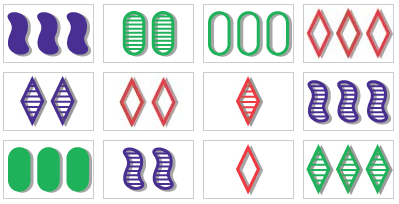
\includegraphics[width=0.5\textwidth]{cards}
\caption{Unas cartas de \SET.}
\end{figure}

\textbf{
Cada carta tiene cuatro atributos: forma, color, relleno y número. Cada uno de los
atributos viene en tres variantes:
}

\begin{tabular}{|c |c|}
\hline
Numero: & 1, 2 o 3.  \\
\hline
Forma: & Diamante, fideo u óvalo.\\
\hline
Color: &Verde, celeste o fucsia.\\
\hline
Relleno: &Vacío, rayado o lleno.\\
\hline
\end{tabular}

Hay exactamente una carta con cada combinación posible de todos los atributos, así que
hay $3^4 = 81$ cartas en el mazo del \SET.

\paragraph
Un \SET~es una familia de tres cartas que cumplen con lo siguiente: \textbf{Las
tres cartas son todas iguales o todas distintas para cada atributo}. Por ejemplo en la
figura 1 las cartas en las posiciones $[1,4]; [2,2]; [3,3]$ forman un \SET, porque son
iguales en color, forma y relleno, pero no se repiten el número. También las que están en
las posiciones $[4,1]; [4,2]; [1,3]$, porque tienen todas el mismo número y todas sus
otras características distintas. Una manera facil y breve de enunciar la regla es que tres
cartas forman un \SET~  si y solo si cada vez que dos cartas comparten una característica,
la tercera también la tiene. 

\paragraph
Es interesante notar que \textbf{dadas dos cartas hay exactamente una carta que, junto con
las dos originales, forman un \SET}: las características de las dos primers determinan la
de la tercera. Como dos cartas definen un \SET, y cada \SET~es determinado por tres pares
de cartas distintos, hay exactamente $\frac{1}{3}\binom{81}{2} = 1080$ \SET's distintos.
Además, cada carta aparece en exactamente 40 \SET's. ¿Por qué?

\paragraph
Para jugar al juego se ponen doce cartas sobre una mesa y todos los jugadores buscan
\SET's al mismo tiempo. Cuando alguien encuentra uno lo retira de la mesa y agregan tres
cartas nuevas. Si no hay \SET's sobre la mesa, se agregan tres cartas más. Es natural
preguntarse entonces

\noindent \textbf{¿Cuántas cartas hay que poner sobre la mesa para estar
seguro de que aparece un \SET~entre ellas?} 

Llamemos $N$ a la respuesta a esta pregunta. Por lo que acabamos de decir $12 < N$. Si
pongo las 81 cartas sobre la mesa, vamos a tener los $1080$ \SET's posibles presentes. Si
retiramos una de las cartas entonces desaparecen los $40$ \SET's que involucraban a esa
carta, pero quedan $1040$ presentes. Siguiendo así vemos que si retiramos 26 cartas
entonces quedan al menos $1080 - 40.26 = 40$ \SET's sobre la mesa, así que $N \leq 55$.
Por otro lado una búsqueda inteligente y breve (o bruta y larga) nos hace llegar a este
conjunto de 20 cartas sin \SET's:

\begin{figure}[h!]
\centering
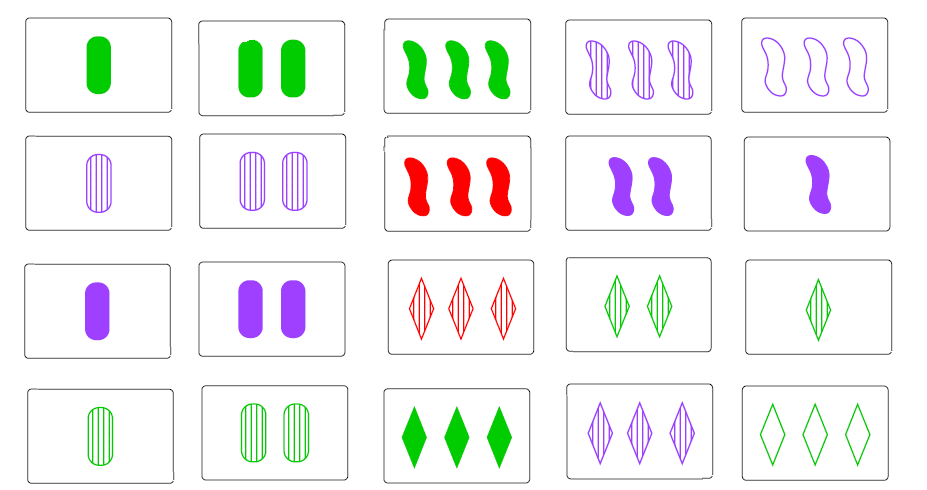
\includegraphics[width=0.85\textwidth]{caps}
\caption{Veinte cartas sin un \SET.}
\end{figure}

Más bruteza con la computadora nos permite concluir que todo conjunto de veintiun cartas
contiene un \SET, así que $N = 21$. Ahora, ¿será que hay algún argumento por el cuál
podemos saber este resultado sin chequear \emph{todos} los casos?

\section{Antes del \SET, el \set.}
\paragraph
La respuesta es que sí, pero el argumento es un poco complicado. Para entenderlo vamos a
considerar primero un caso más sencillo. Vamos a jugar al \set, que es como el \SET, pero
las cartas tienen solo dos atributos: forma y relleno. Para jugar al \set~usamos un mazo
parecido, con nueve cartas:
\begin{figure}[h!]
\centering
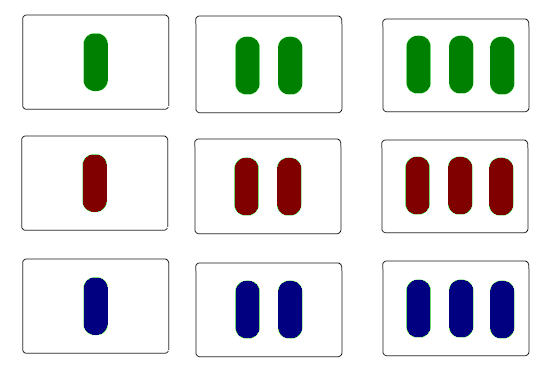
\includegraphics[width=0.5\textwidth]{ov-rojo}
\caption{Cartas de \set.}
\end{figure}

\paragraph
Vamos a pensar en nuestro problema en el caso del \set: Llamamos $N_2$
al menor número de cartas que hay que poner sobre la mesa para asegurarse de que exista un
$\set$. Notar que tres cartas alineadas siempre forman un \set. Para fijar ideas, miremos
todos los \set's que incluyen al óvalo vacío. Son las tres lineas que salen del vértice
superior, más el \set~que forman las tres cartas encerradas en un círculo:

\begin{figure}[h!]
\centering
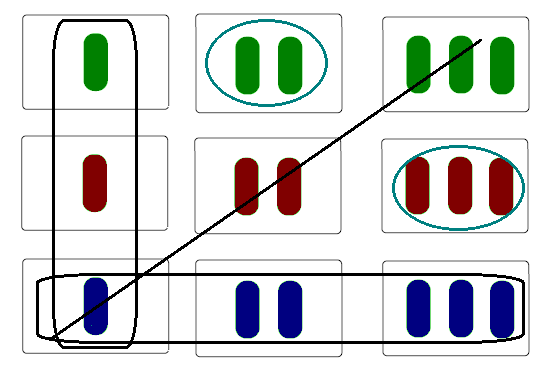
\includegraphics[width=0.5\textwidth]{ov-rojo-s}
\caption{Los \set~que incluyen a la primera carta.}
\end{figure}

En cierta forma las tres cartas encerradas también forman una línea recta. En el diagrama
empezamos con las cartas con relleno vacío, pero si empezamos por las de relleno rayado,
obtenemos un diagrama muy parecido donde este tercer \set~sí forma una linea recta.

\begin{figure}[h!]
\centering
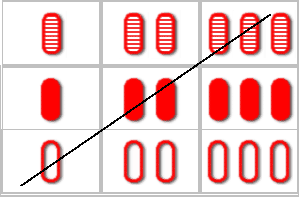
\includegraphics[width=0.5\textwidth]{ov-rojo-2}
\caption{Un diagrama parecido.}
\end{figure}

\paragraph
Hay un truco muy interesante que permite entender este asunto de los \set's y las lineas
rectas. Sea $\FF_3$ el cuerpo de $3$ elementos. A cada carta de la figura $4$ le asignamos
un punto del espacio vectorial $\FF_3^2$, de la siguiente manera:
\begin{tabular}{|c|c|c|}
\hline
(0,0) & (0,1) & (0,2) \\
\hline
(1,0) & (1,1) & (1,2) \\
\hline
(2,0) & (2,1) & (2,2) \\
\hline
\end{tabular}

Ahora vemos que los \set's que incluyen a la carta en la posición $(0,0)$ son los
siguientes:
\begin{align*}
\{(0,0); (0,1); (0,2)\} && \{(0,0);(1,0);(2,0)\} && \{(0,0);(1,1); (2,2)\} &&
\{(0,0);(1,2);(2,1)\}.
\end{align*}
Estos conjuntos son exactamente los subespacios de dimensión 1 de $\FF_3^2$. Notar que sus
ecuaciones son respectivamente $x = 0; y = 0; y - x = 0; y + x = 0$. De la misma forma se
puede ver que, con esta correspondencia, todo \set~defne una recta afín (que no pasa
necesariamente por el orígen) en el espacio $\FF_3^2$. Una familia de cartas que no
contenga ningún \set~se corresponde entonces con un conjunto que no contenga ninguna recta
afín.

\paragraph
\label{2-cap}
Un subconjunto de $\FF_3^2$ que no contiene ninguna linea se llama un $2$-cap. Con nuestra
equivalencia, un $2$-cap es lo mismo que un conjunto de cartas que no contiene \set's, así
que el siguiente resultado debería ser muy interesante:
\begin{Proposition*}
Un $2$-cap tiene a lo sumo 4 elementos.
\end{Proposition*}
\begin{proof}
Notar que todo subconjunto de un $2$-cap es un $2$-cap, así que basta ver que no existen
$2$-caps de cinco elementos. Supongamos que sí existe uno, y llamémoslo $C$. Ahora
observemos que si $C$ es un $2$-cap y $p \in \FF_3^2$, entonces $C - p$ también es un
$2$-cap: si $C - p$ contuviera la linea $L$ entonces $C$ contendría a la linea $L + p$, lo
cual contradice que $C$ sea un $2$-cap. Tomando $p \in C$, podemos cambiar $C$ por $C -
p$, que contiene al $(0,0)$, así que sin pérdida de generalidad podemos suponer que $(0,0)
\in C$.

Ahora queremos hacer otra observación: si $T: \FF_3^2 \to \FF_3^2$ es un isomorfismo lineal,
entonces manda lineas rectas en lineas rectas, así que también manda $2$-caps en $2$-caps.
Como $C$ tiene cinco puntos, puedo tomar dos puntos $p, q \in C$ distintos del $(0,0)$, y
como $p, q$ no están alineados con el origen, son linealmente independientes (verificar!)
y forman una base de $\FF_3^2$; por lo tanto existe un isomorfismo lineal $T: \FF_3^2 \to
\FF_3^2$ tal que $T(p) = (1,0); T(q) = (0,1)$. Cambiando $C$ por $T(C)$ si es necesario,
vemos que una vez más podemos suponer sin pérdida de generalidad que nuestro $2$-cap
contiene al conjunto $\{(0,0), (1,0), (0,1),\}$ y otros dos puntos, $x, y$. Como $(0,0),
(1,0)$ y $(2,0)$ son colineales, está claro que $(2,0) \notin C$, y de la misma manera se
descarta $(0,2)$ y $(2,2)$. Resulta entonces que $x,y \in \{(1,1); (2,1); (1,2)\}$, y es
facil ver que toda elección posible lleva a una contradicción. Luego no existen $2$-caps
de cinco elementos.
\end{proof}
De esto se deduce inmediatemente que poniendo 5 cartas del mazo de \set~ sobre la mesa
vamos a tener al menos un \set~ presente, es decir que $N_2 = 5$.

\section{Después del \set, el \Set}
\paragraph
Aumentemos un poco la complejidad del problema. Consideremos ahora el \Set, que es como el
\SET, solo que las cartas tienen \emph{tres} atributos. El mazo es de la siguiente forma:

\begin{figure}[h!]
\centering
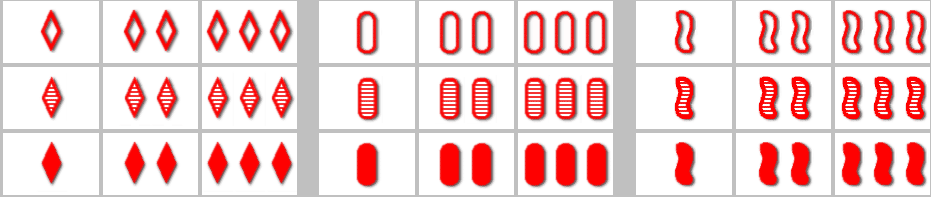
\includegraphics[width=0.85\textwidth]{Set}
\caption{Cartas de \Set.}
\end{figure}

que identificamos con los puntos de $\FF^3_3$ de manera obvia. También sigue valiendo que
toda recta afín es un \Set, y que todo \Set~se corresponde con una recta afín. Para
verificarlo, basta comprobar dos cosas
\begin{enumerate}
\item Tres puntos $P,Q,R$ de $\FF_3^n$ son colineales si y solo si $P + Q + R = 0$.
\item Tres números $\alpha, \beta, \gamma \in \FF_3$ tales que $\alpha + \beta + \gamma =
0$ son o los tres iguales o los tres distintos.
\end{enumerate}
Al combinar ambos ítems vemos que tres puntos son colineales en $\FF_3^n$ si y solo si,
para cada $i = 1, 2, \ldots, n$, las $i$-ésimas coordenadas de los puntos son todas
iguales o todas distintas. Queda al lector convencerse de que esto se traduce en que todo
$\Set$~se corresponde con exactamente una linea afín en $\FF_3^3$.

\paragraph
Una vez más nos interesa calcular cuántas cartas de \Set se necesita poner sobre la mesa
para estar seguro de que hay al menos un \Set presente. Equivalentemente, podemos
preguntarnos cuál es el número de puntos del $3$-cap más grande; por supuesto un $3$-cap
es un conjunto de puntos en $\FF_3^3$ que no contiene ninguna linea. Otra vez, es facil
encontrar un $3$-cap de nueve elementos, como el siguiente

\begin{figure}[h!]
\centering
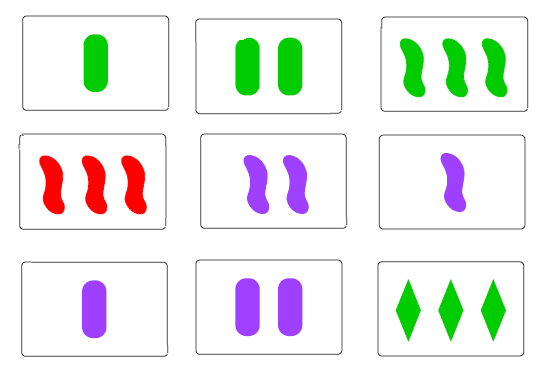
\includegraphics[width=0.85\textwidth]{caps2}
\caption{Un $3$-cap de $9$ puntos.}
\end{figure}

\begin{Proposition}
\label{3-cap}
  Un $3$-cap tiene a lo sumo $9$ elementos.
\end{Proposition}
Daremos dos pruebas de este hecho
\begin{proof}
  Notar primero que si intersecamos un $3$-cap con cualquier plano, obtenemos un $2$-cap
  para ese plano. Supongamos ahora que $C$ es un $3$-cap que contiene diez puntos, y
  miremos los $2$-caps $C_i = C \cap \{x = i\}$ para $i = 0, 1, 2$. Claramente $C = C_1
  \cup C_2 \cup C_3$, y como cada $C_i$ tiene a lo sumo cuatro puntos y $C$ tiene
  exactamente diez, está claro que existe un $i$ tal que $C_i$ tiene o dos o tres puntos.
  Sin pérdida de generalidad (completar!) podemos suponer que $(0,0,0), (0,1,0) \in C_0$ y
  que $C \setminus C_0$ tiene al menos siete puntos, que llamamos $P_1, \ldots, P_7$.

  Sabemos que para cada $i$ los puntos $(0,0,0), (0,1,0), P_i$ no estan alineados, así que
  $H_i = \langle (0,1,0), P_i\rangle$ es un hiperplano \emph{distinto de $C_0$} que
  contiene a estos tres puntos. Es facil ver que hay exactamente cuatro planos que
  contienen a $(0,0,0), (0,1,0)$, así que el conjunto $\{H_i \mid i = 1, \ldots, 7\}$
  tiene a lo sumo tres elementos, y eso implica que hay repeticiones en la lista de los
  $H_i$'s. Sin pérdida de generalidad podemos suponer que $H_1 = H_2 = H_3$, y llamamos
  simplemente $H$ a este espacio. Por definición de $H$ sabemos que $\{(0,0,0); (0,1,0);
  P_1; P_2; P_3\} \subset C \cap H$, es decir que $C \cap H$ es un $2$-cap con al menos
  cinco elementos, lo que contradice la Proposición \ref{2-cap}.
\end{proof}

\paragraph
La demostración anterior es puramente combinatoria, en el sentido de que solo involucra
contar las cosas de manera inteligente. Con un razonamiento similar se puede dar una cota
para el problema del \SET, pero no la mejor. La siguiente demostración de la Proposición
\ref{3-cap} es un poco más complicada, pero se puede generalizar a dimensiones superiores.
\begin{proof}[Otra Demostración]
  Supongamos otra vez que tenemos un $3$-cap de diez elementos, llamado $C$. Dado un
  plano $H$, podemos descomponer $\FF_3^3$ como la unión de $H$ y otros dos
  planos paralelos, digamos $H'$ y $H''$. Hay entonces ocurre una de dos cosas:
  \begin{itemize}
  \item Dos de los planos tienen cuatro puntos de $C$ y el otro dos;
  \item Uno de los planos tiene cuatro puntos de $C$, y los otros dos tienen tres.
  \end{itemize}
  Notamos $x_{442}$ al número de planos que caen en el primer caso, y $x_{433}$ a
  los que caen en el segundo caso. Entonces $x_{433} + x_{442} = 13$, que es el número
  total de planos de $\FF_3^3$.
  
  Vamos a buscar una segunda ecuación involucrando las variables $x_{433}$ y $x_{442}$.
  Para ello vamos a contar de cuántas maneras se pueden formar pares $(H, \{x,y\})$ de
  forma que $H \subset \FF_3^3$ es un plano afín (no pasa necesariamente por el orígen) y
  $\{x,y\} \subset C \cap H$. Estos pares se llaman \emph{hiperplanos 2-marcados}, y
  llamamos $M$ al número de hiperplanos 2-marcados. Como mencionamos antes, todo par de
  puntos de $\FF_3^3$ pertenece a exactamente cuatro hiperplanos, así que eligiendo dos
  puntos de $C$ podemos formar cuatro hiperplanos 2-marcados distintos, por lo que $M =
  4\binom{10}{2} = 180$. Por otro lado, si tenemos un plano del tipo $x_{442}$, entonces
  podemos construir $\binom{4}{2} + \binom{4}{2} + \binom{2}{2} = 13$ planos 2-marcados
  distintos (por qué?) y si tenemos uno de tipo $x_{433}$ podemos construir $\binom{4}{2}
  + \binom{3}{2} + \binom{3}{2} = 12$ hiperplanos 2-marcados. Estas son todas las
  variantes posibles de hiperplanos 2-marcados, contadas sin repetición (por qué?), así
  que $12x_{433} + 13 x_{442} = 180$.

  Tenemos entonces el sistema $\begin{cases} x_{433} + x_{442} & = 13 \\ 12x_{433} +
  13x_{442} &= 180 \end{cases}$, de donde se deduce que $x_{433} = - 11$, lo que es
  absurdo ya que claramente $a$ debería ser un número natural.
\end{proof}
\end{document}
